\chapter{\pbox: a Balanced Hardware Design for Parameter Servers at Rack-Scale}
\label{sec:phub}
We now describe \pbox, the solution to inefficient distributed training for clusters with a flat network topology (rack-level). \pbox provides a re-design of a PS at the hardware level, and mostly applies to situations where the user assumes full control over the cluster. We start with the current problem with the PS software and hardware that runs it.

\begin{table}
        \centering
        \footnotesize
	\begin{tabular}{|c|c|c|c|c|}
		\hline
		Network   & CC & CS & NCC & NCS\\
		\hline
		ResNet 269    & 122   & 31   & 140    &  17   \\
		\hline
		Inception & 44   &  11  &  50   &  6  \\
		\hline
		GoogleNet & 40   &  10  &  46   &  6  \\
	
		\hline 
		AlexNet   & 1232  &  308  & 1408    &  176  \\
		\hline
	\end{tabular}
	\caption{Estimated bisection bandwidth (Gbps) lower bound on the PS side for hiding communication latency in a small cluster of 8 nodes with GTX 1080 Ti.}
	\label{table:bwReqDC}
\end{table}

\section{Insufficient Bandwidth and Overprovisioned Compute Resources in Rack-Scale Clusters}
Centralized PSs have lower cost than NCS PSs, and half of the bandwidth stress compared to CS PSs on each interface card. Thus it is desirable to have a centralized reduction entity at rack level. However, scaling a centralized PS to rack scale is challenging~\cite{firecaffe}.
%Because they dedicate their full bandwidth to the PS process, centralized PSs are bandwidth efficient without the extra hardware cost for non-colocated sharded PSs. They are also compute efficient when not overwhelmed~\cite{firecaffe}. However, while optimizations in \mysection\ref{sec:commonOptimizations} benefit sharded servers, they have only limited effect on the throughput of a centralized PS. 
%The root cause is hardware imbalance in resource allocation of the host machine.
The root cause is hardware imbalance in the allocation of computation and communication resources in the host: centralized PSs usually run on the same hardware configuration as a worker, which have only one or two network interfaces. This implies incast congestion from their high bandwidth usage when serving multiple workers, starving the compute units. We profiled the training of multiple DNNs of different model sizes and computation-to-communication ratios. Our setup used 8 workers and 8 CS PSs. We observed \textit{it was nearly impossible to eliminate communication latency in cloud-based training due to limited network bandwidth.} We estimated the minimum bandwidth requirement to fully hide communication latency in the network as follows: given a model size of $M$, and $T$ time for each iteration, with $N$ workers participating, the network should at least be able to send and receive model updates within the computation time (assuming infinitely fast PSs and that sending/receiving could fully overlap). Figure \ref{fig:pssetups} gives an analytical lower bound of \textit{per host bandwidth}, and Table \ref{table:bwReqDC} shows the required bandwidth for various DNNs: DNNs demand more bandwidth than mainstream offers (typically 10 Gbps). 

%Hardware imbalances result from vastly different computation and communication resources in a machine, which is in turn related to how centralized PSs are deployed. Centralized PSs usually run on the same hardware as a worker and have only one or two network interfaces. This implies incast congestion from their high bandwidth usage (Table \ref{table:bwReqDC}) when serving multiple workers, starving the compute units. 

%Existing frameworks also cannot efficiently use full hardware, even if multiple interfaces are present (for example, TensorfFlow and \mxnet can only use multiple interfaces by spawning multiple PS processes), let alone understanding the topology of the underlying hardware to balance workload in each interface, processor core and NUMA domain.

One trivial solution would be to simply use interfaces with higher bandwidth. However, even in the best case, a single network interface is not capable of saturating memory or PCIe bandwidth. A single network interface also causes serialization delay and further imbalance across NUMA domains in a typical server. %It is not possible to fully utilize the entire server without balancing these resources.

%The solution may seem trivial: just add more interfaces, or use interfaces with higher capacity. These, however, are not enough. First, most parameter server implementations (TensorFlow, \mxnet and etc) do not allow use of multiple interfaces in a single parameter server process instance. To support that, the software stack must understand the topology of the underlying system and produce a balanced scheme across multiple interfaces with minimum polling overhead; second, existing single interface is unlikely able to match the memory bandwidth nor the PCIe bandwidth, and they can still cause serialization delay, further causing imbalance across NUMA domains on typical server systems.

%Software changes alone is not enough to scale training throughput on a typical centralized parameter server, because the hardware offered is inbalanced itself: the provisioned network bandwidth is vastly smaller than available memory bandwidth.
%Therefore, a hardware design that optimizes balance is needed to fully scale a centralized PS. 

\section{\pbox Architecture}
This section describes \pbox, our \textit{balanced parameter exchange system}. We maintain that a centralized system, when architected properly, can provide high throughput, low latency, sufficient scalability for a rack, and low cost. We focus on the hardware side of \pbox, and in the next section, we detail the software side.

We prototyped \pbox using an off-the-shelf server platform that was configured to our requirements. Our goal was to balance IO and memory bandwidth; our prototype system had memory bandwidth of 120 GB/s and theoretical overall bidirectional IO bandwidth of 140 GB/s. To fully utilize resources, \pbox needed a matching network capability, which we provided by using multiple network interfaces. Figure \ref{fig:phub} shows the resulting \pbox design. The system includes 10 network interfaces, each of 56 Gbps link speed, connected to a switch. This uses all PCIe bandwidth on our dual socket prototype and provides roughly 136 GB/s bandwidth once IB and PCIe framing overheads are taken into account, balancing IO and memory bandwidth.

\begin{figure}[t!]
	\centering
	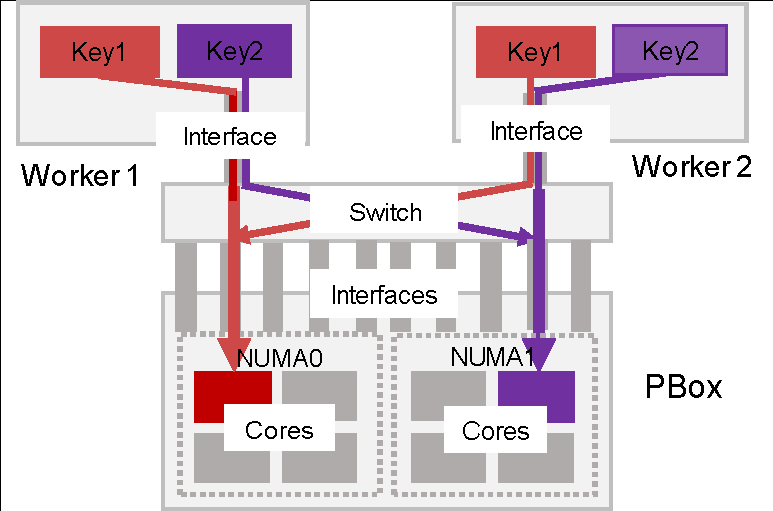
\includegraphics[width=.6\linewidth,trim=2 1 1 1,clip]{Figures/PHubOverview.pdf}
	\caption{The \pbox architecture}
	\label{fig:phub}
\end{figure}



\begin{figure}[t!]
	\centering
	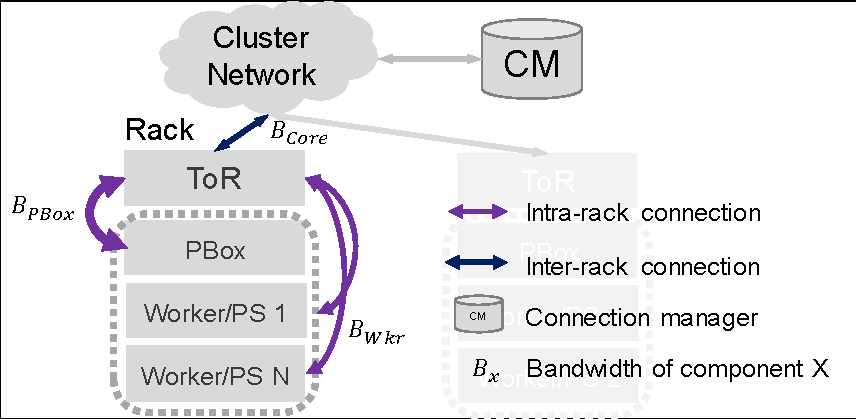
\includegraphics[width=.7\linewidth,trim=3 1 1 2,clip]{Figures/PBoxDeployment.pdf}
	\caption{\pbox deployment scheme}
	\label{fig:pBoxDeployment}
\end{figure}


\section{Multi-Rack Deployment and Topology-Aware Reduction}
\label{sec:hierarchicalReduction}
To extend service coverage of a single \pbox device, we associate a \pbox with a ToR during deployment, for two reasons. First, full bisection bandwidth is achievable for machines in the same rack, making it ideal for a central reduction entity as \pbox, while oversubscription occurs between the ToR and the cluster network. Second, as we show later, a single \pbox has enough scalability for a typical rack of worker machines.

When provisioned in each rack (Figure \ref{fig:pBoxDeployment}), \pbox{}es can form an array of sharded PSs, or run a \textit{hierarchical reduction} algorithm for a training task that spans multiple racks through the coordination of a connection manager. Hierarchical reduction works in three steps: first, each \pbox centrally aggregates gradient updates from workers in the same rack; then, the \pbox{} nodes start cross-rack aggregation and compute globally aggregated gradients; finally, each per-rack \pbox runs an optimizer on this gradient and broadcasts the new weights back to local workers.

Hierarchical reduction trades off more rounds of communication for lower cross-rack traffic ($1/N$ with N-worker racks). We can determine when hierarchical reduction is potentially beneficial with the simple model below:
%\[	max(\frac{N-1}{B_{bn}}, \frac{1}{B_{Wkr}})  > max(\frac{1}{B_{Wkr}}, \frac{N}{B_{PBox}}) + C\]

\begin{align*}
	 \frac{N(R-1)}{RB_{Core}} >  max(\frac{N}{B_{PBox}}, \frac{1}{B_{Wkr}}) + C
\end{align*}
%\[\]

where $B_{PBox}, B_{Core}$ and $B_{Wkr}$ are the bandwidths of a \pbox, the network core, and a worker, and $R$ is the number of racks. When the condition is true, this means the time to perform cross-rack transfer is larger than the added latency of a two-level reduction, which consists of a per-rack local aggregation that happens in parallel and an inter-rack communication (with cost $C$) done with either sharded PSs ($C=\frac{r-1}{rB_{bn}}$, where $B_{bn} = min(B_{PBox}, B_{Core})$) or a collectives operation (e.g., $C\approx\frac{r-1}{rB_{bn}}$ with racks forming a ring). $C$ can be directly measured, and $B_{Core}$ can be effectively probed by using~\cite{hu2002estimating,hu2003evaluation}.
